\documentclass[a4paper,english]{article}
\usepackage{graphicx}
\usepackage{listings}
\usepackage{amsmath}
\usepackage{multirow}

%% Use utf-8 encoding for foreign characters
%%\usepackage[T1]{fontenc}
%%\usepackage[utf8]{inputenc}
%%\usepackage{babel}
%%
%%%% Vector based fonts instead of bitmaps
%%\usepackage{lmodern}
%%
%%%% Useful
%%%\usepackage{fullpage} % Smaller margins
%%\usepackage{enumerate}
%%
%%%% Theorem
%%\usepackage{amsthm}
%%
%%%% More math
%%\usepackage{amsmath}
%%\usepackage{amssymb}
\lstset{
  breaklines=true,
  postbreak=\mbox{{$\hookrightarrow$}\space},
}

%% Document Header
\title{Section2}
\author{Elliott Ashby}
\date{\today}

\begin{document}
    \maketitle
    \section{q1}
        \lstinputlisting[language=Python, lastline=69]{./2_1.py}
        \begin{center}
        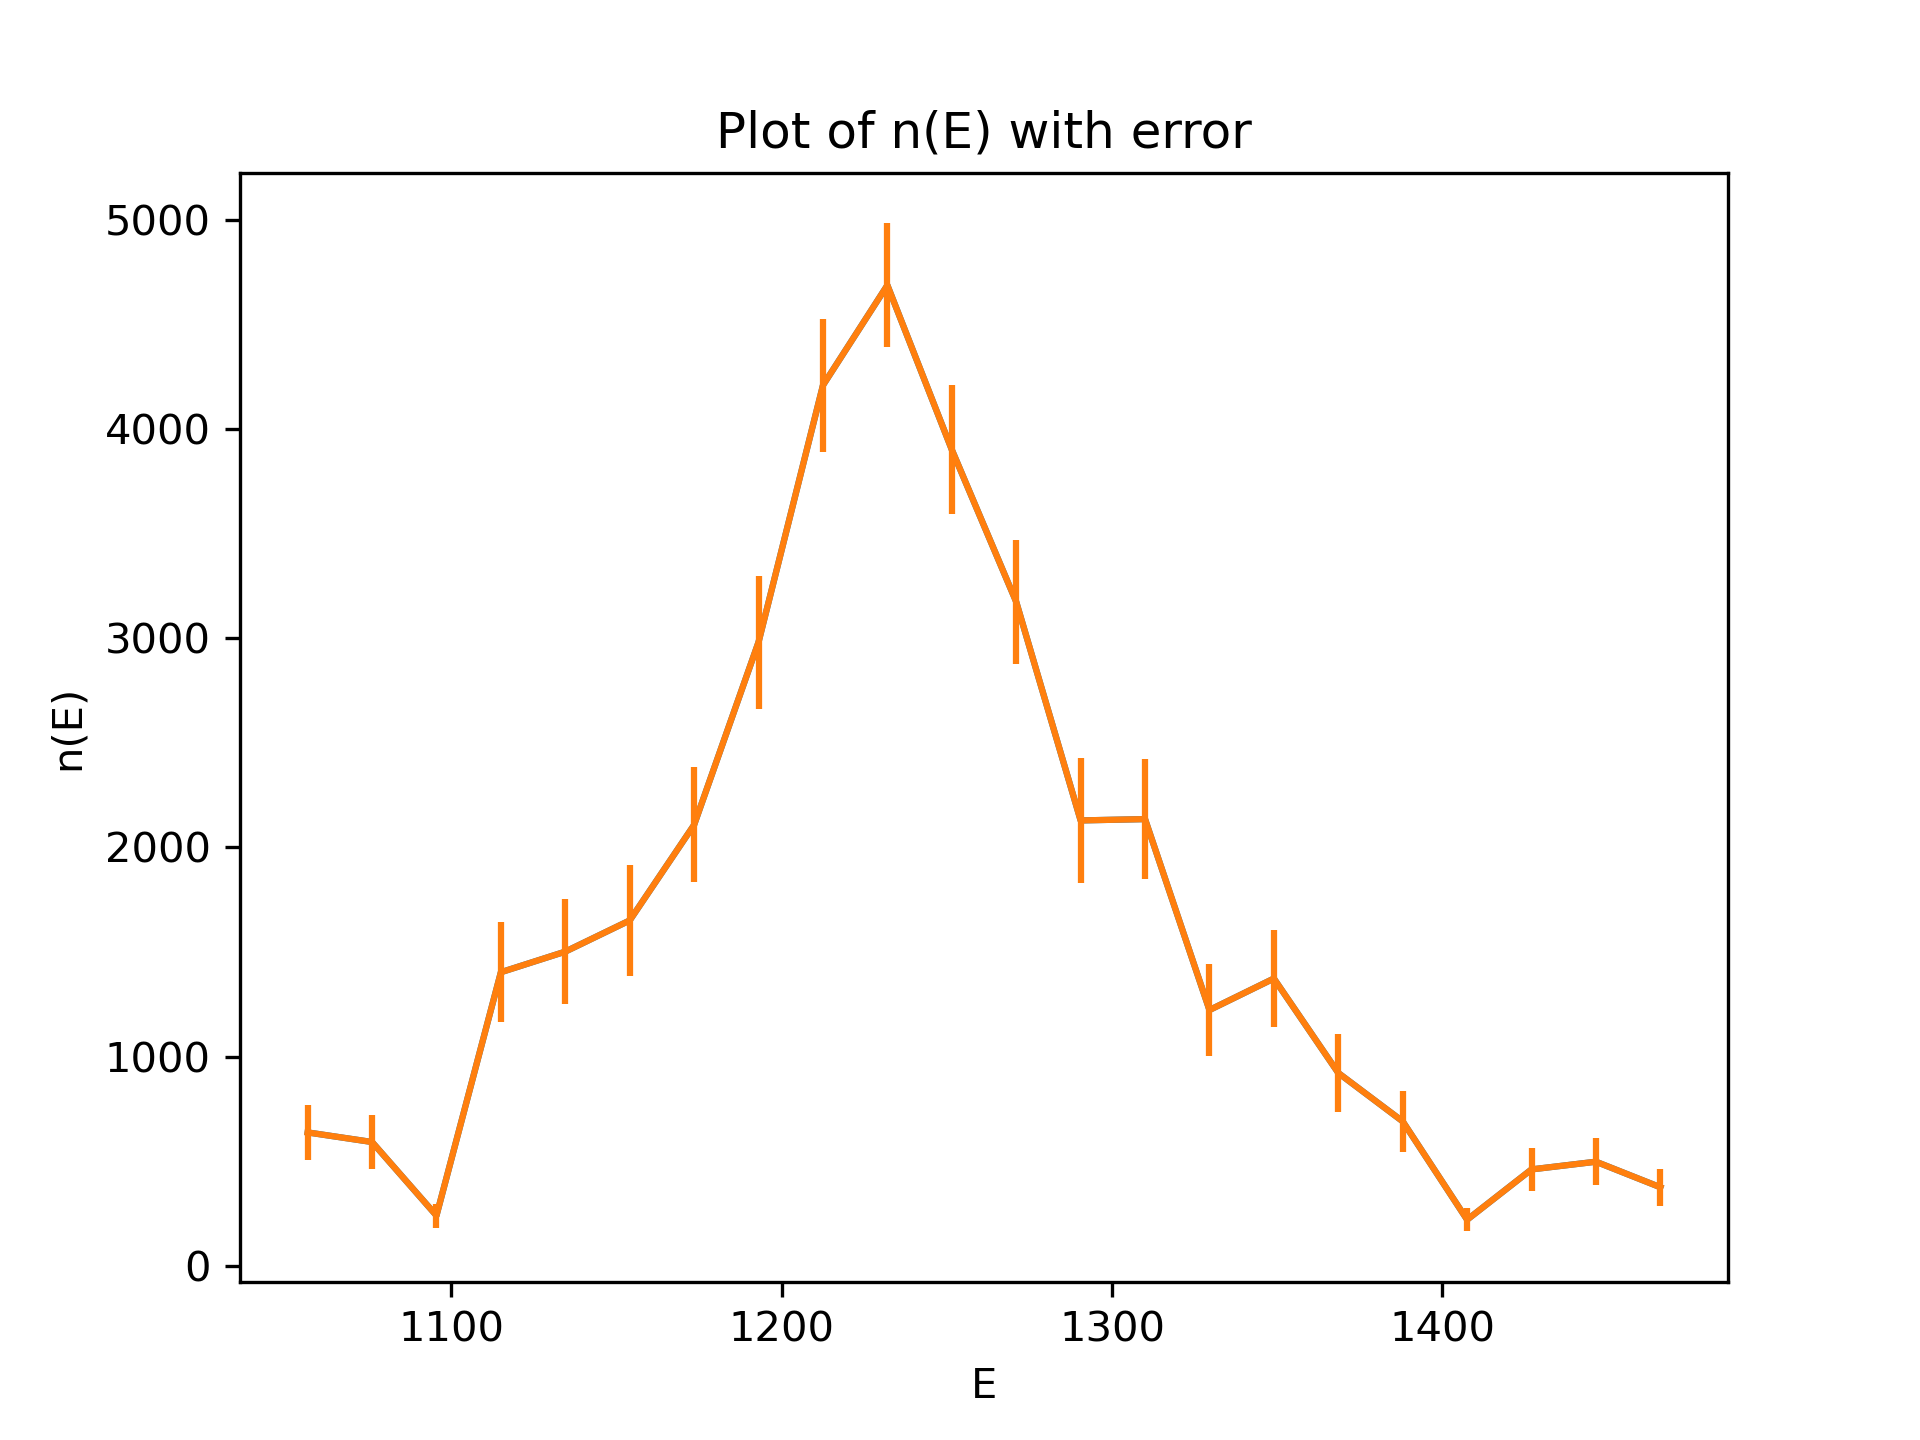
\includegraphics[scale=0.8]{./2_1.png}
        \end{center}
    \section{q2}
        As E increases from 1000 n(E) increases at an increasing rate
        until around 1200 where the gradient change decreases to a peak at 
        around 1250. This shape is mirrored on the other side ending around
        1500.
    \section{q3}
    \begin{center}
    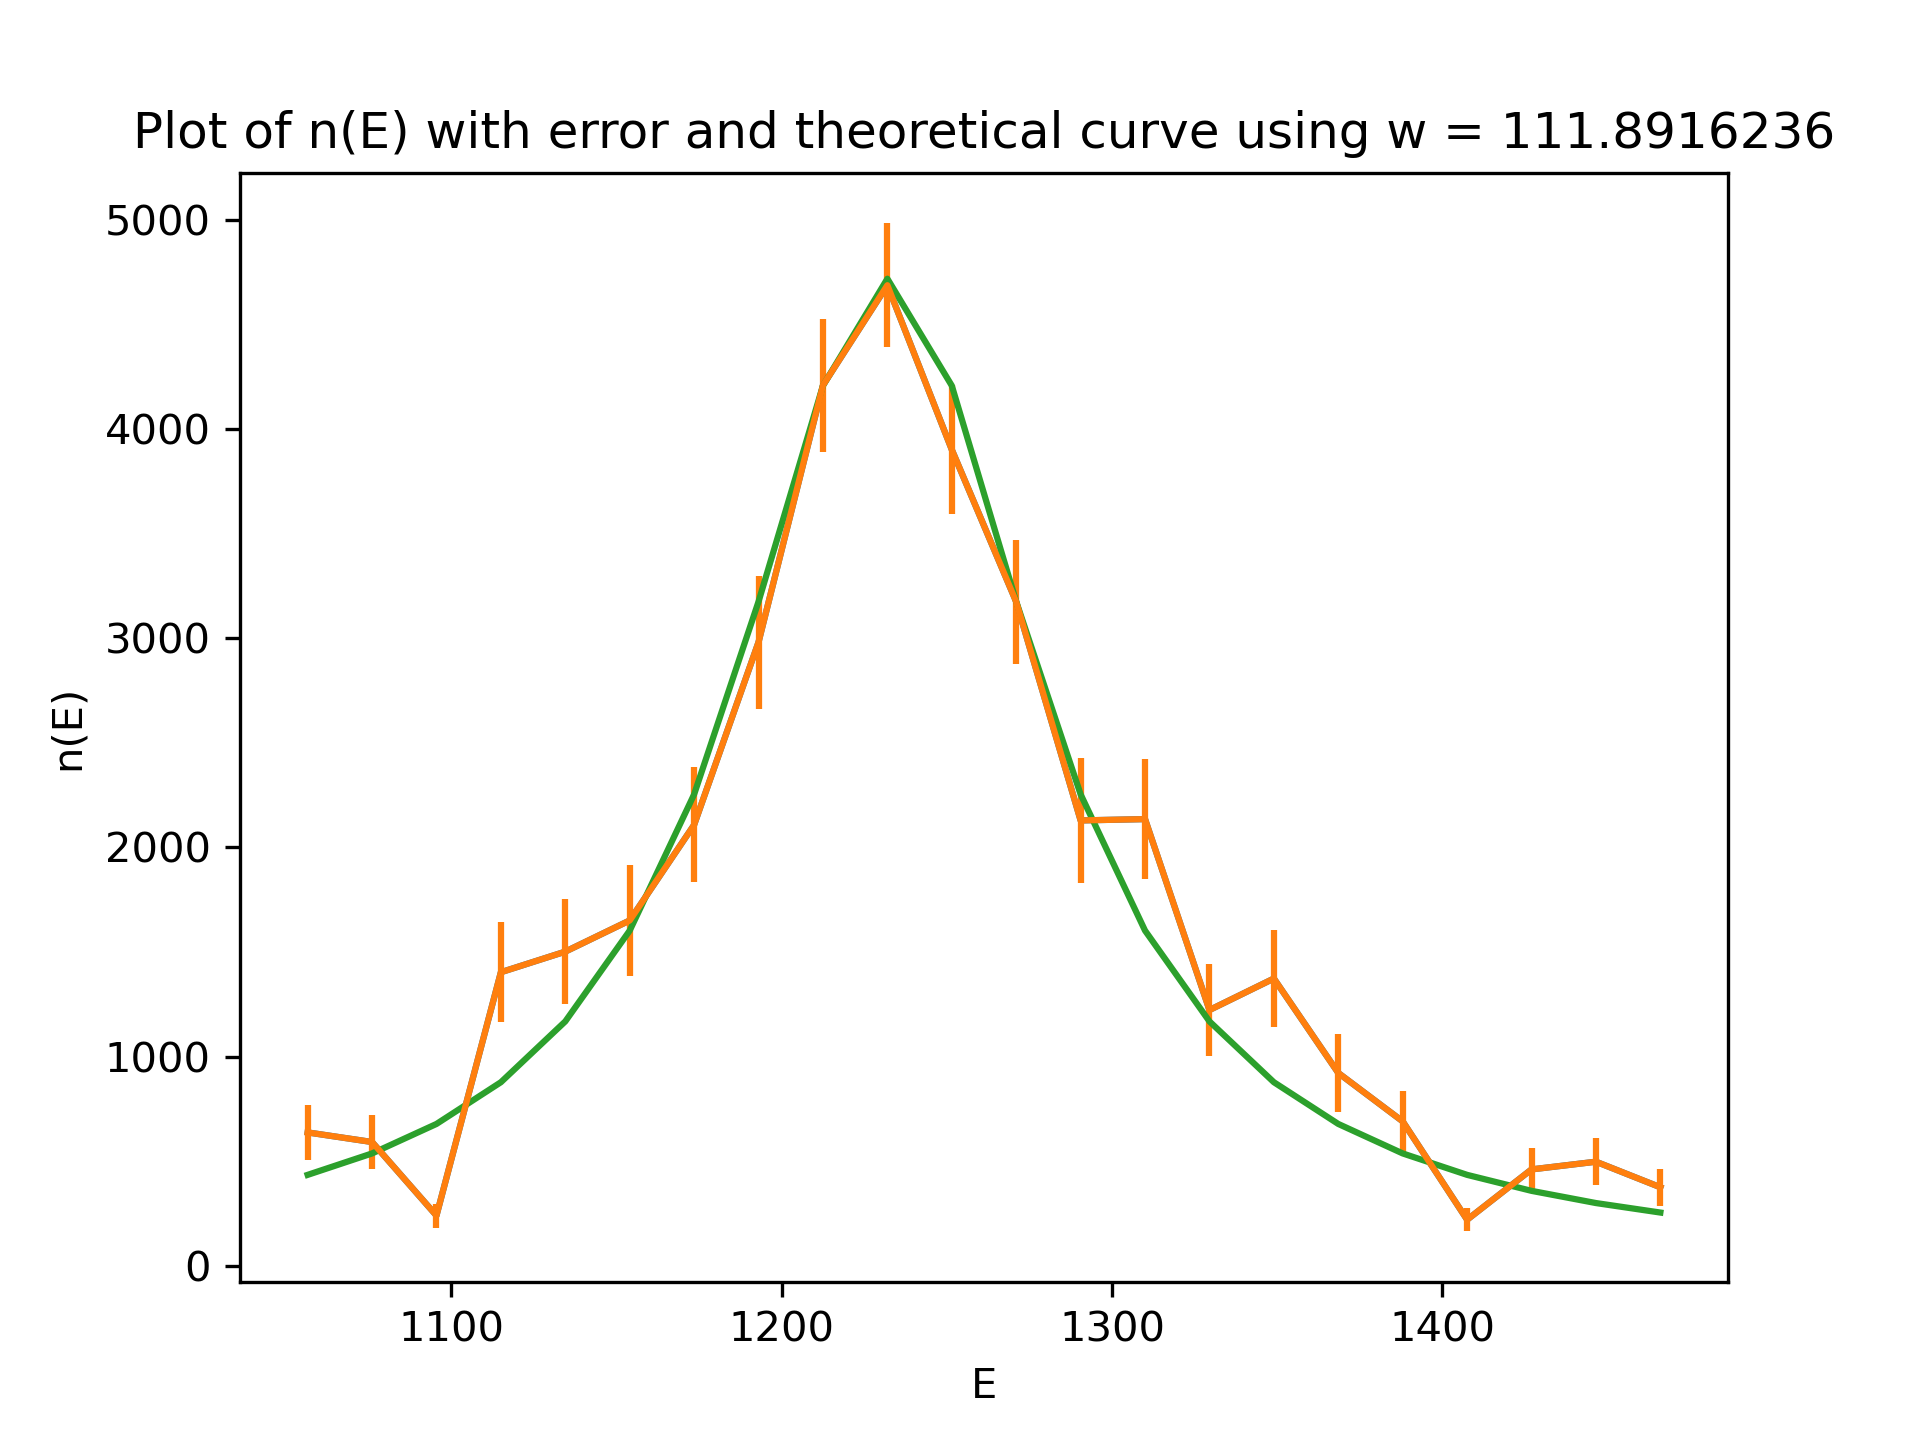
\includegraphics[scale=0.8]{./2_3th.png}
    \end{center}
        \begin{equation}
            w = \frac{600\sqrt{163}}{\sqrt{4687}}
        \end{equation}
        Changing $w$ effects the maximum value of the peak of the theoretical curve
        without changing the minimum values at roughly $n(E) = 500$. Increasing $w$
        decreases the maximum (since $w^2$ is divided by in $n(E)$). Whereas decreasing
        $w$ increases the maximum of $n(E)$.
    \paragraph{Bonus}
        \hfill \break
        \lstinputlisting[language=Python, firstline=72, lastline=90]{./2_1.py}
        Manually using trial and error to reduce the discrepancy results in a minimum discrepancy of 86.76
        which is when $w = 113.15$. The method used is just iterating on the 
        value of $w$ and returning the value of the discrepancy each time as seen in the "minimum\_discrepancy" function.
        \newline Using gmin() on the discrepancy function reveals a minimum $w$ of 
        113.14847521305097 where the discrepancy is 86.76529920076851.
        Using these values in a plot yields:
        \begin{center}
        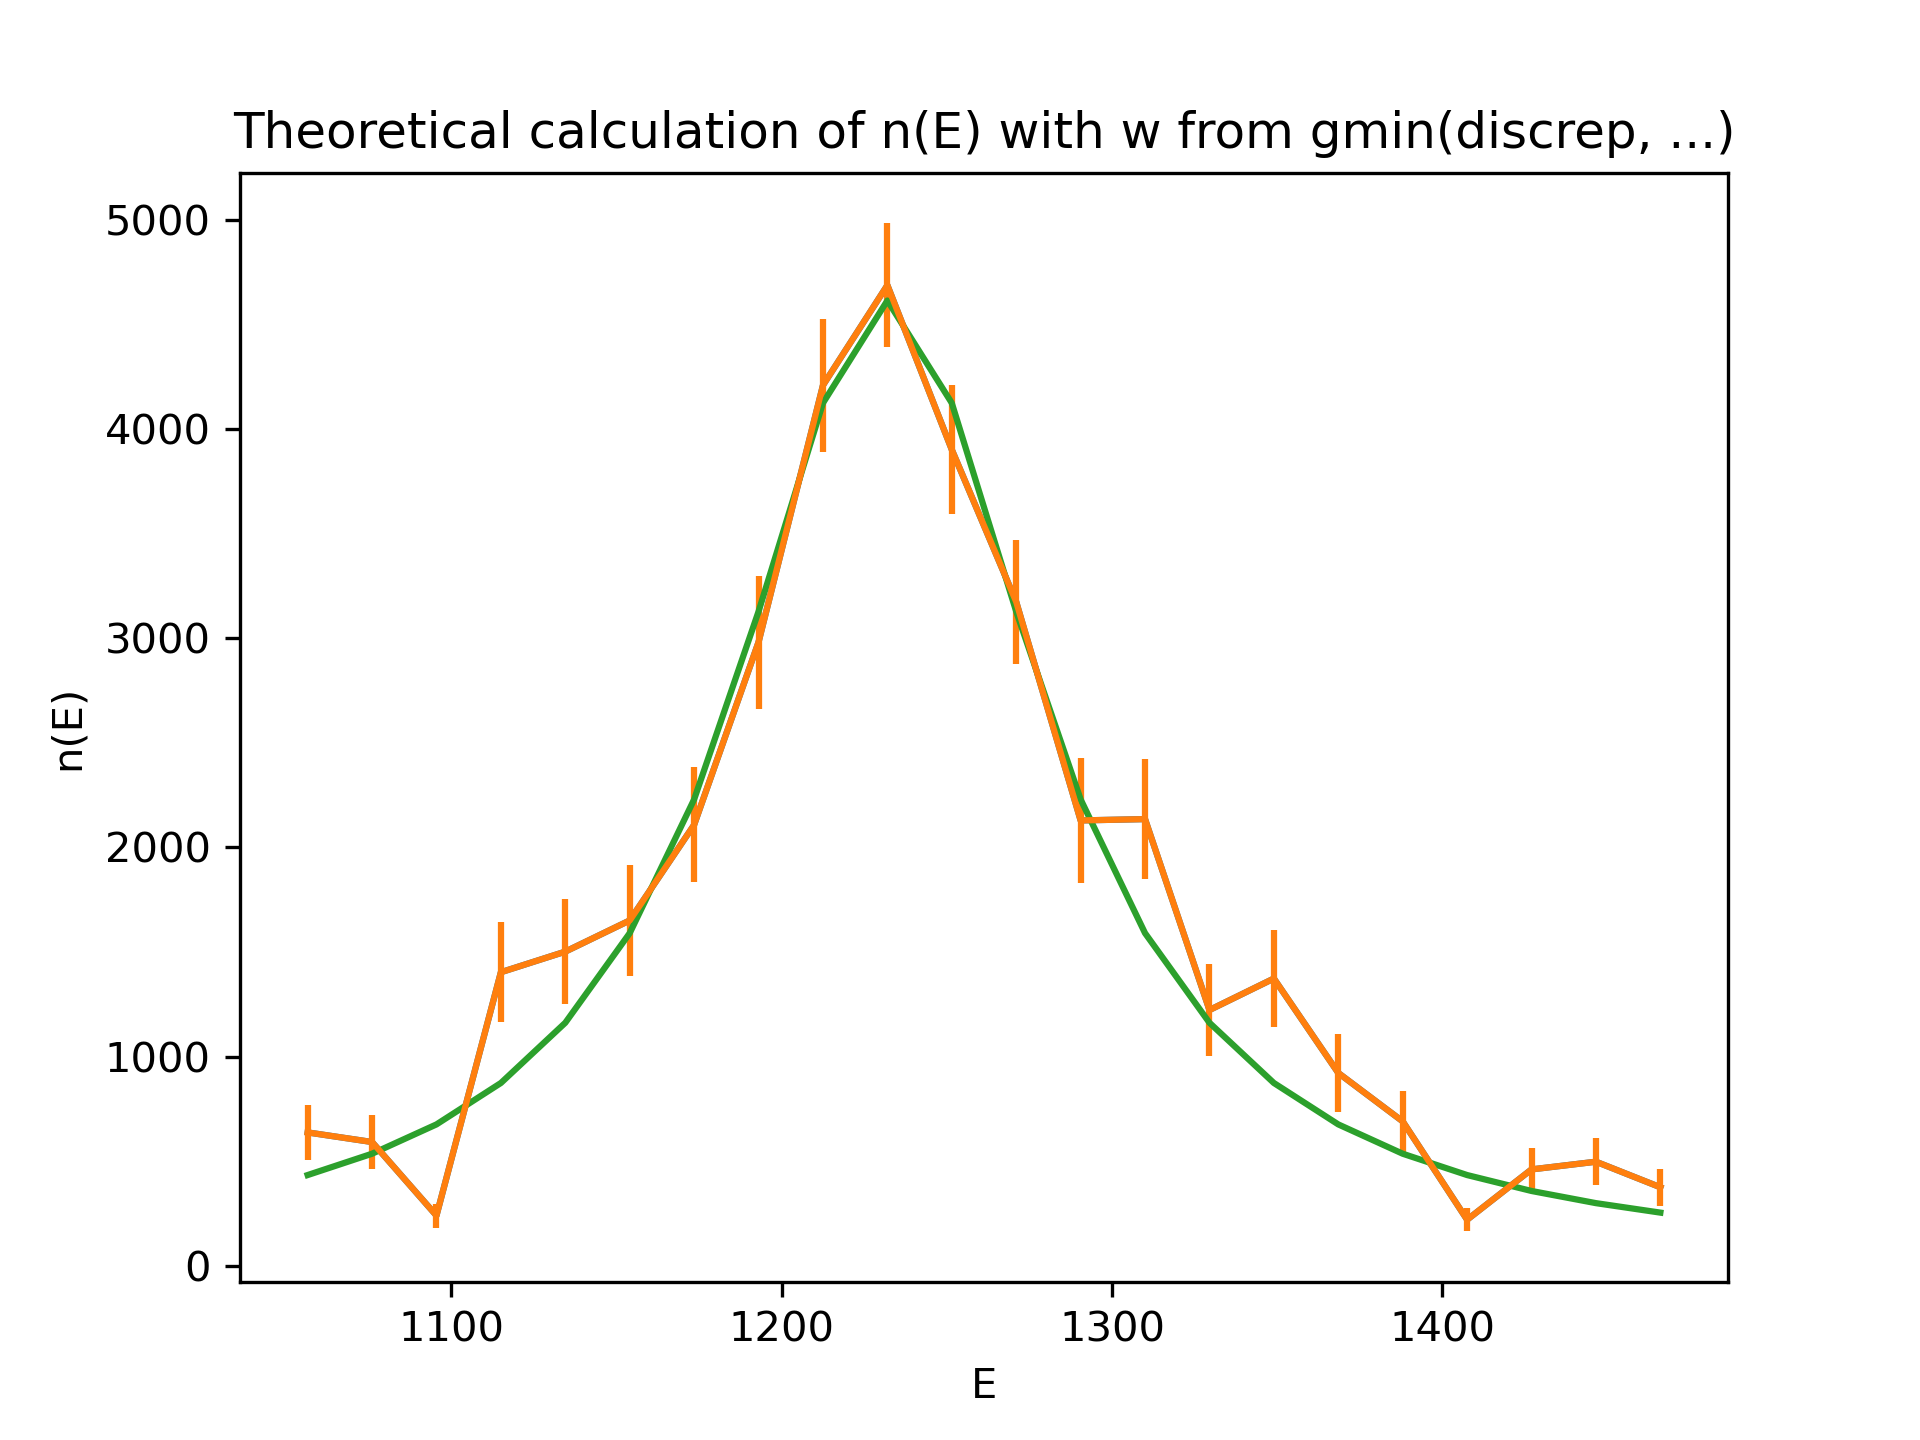
\includegraphics[scale=0.8]{./2_5.png}
        \end{center}
    \section{q4}
        \lstinputlisting[language=Python]{./2_4.py}
        This function takes in the values of the residuals and their errors and 
        returns a sum over each residual divided by their error squared.
    \section{q5}
        \lstinputlisting[language=Python, firstline=84, lastline=87]{./2_1.py}
        This outputs a value of $w$ of 113.14847521 with an uncertainty of 4.84317108
        (This is the value of $w$ that minimises the discrepancy function which was found with the method
        in my bonus section.)

    \section{q6}
        \lstinputlisting[language=Python, firstline=93, lastline=124]{./2_1.py}
        We implement the algorithm described in the question. We start with finding the $w$ of each individual student in the function student, this returns a value of $w$ calculated from a curve fit of randomized values in the shape of a normal distribution with mean and variance defined by data1.txt. \newline
        We then define an all\_students function which takes in the number of students and the data from data1.txt where we append every students individual value of $w$ into a new list. From this we can find the standard deviation using stdev. \newline
        This function then returns the mean of all students $w$ values and the standard deviation of all students $w$ values along with the raw list of $w$. \newline

        Using this algorithm we find that the mean of all students $w$ values is: 
        \begin{center}
            $113.20577213567762 \pm 2.278191315242165$
        \end{center}
        Obviously, since we are using a random number generator to generate the values of $w$ for each student, the values of $w$ will change each time the program is run. However, the mean and standard deviation of the values of $w$ will remain roughly the same.
    
    \section{q7}
        \begin{center}
        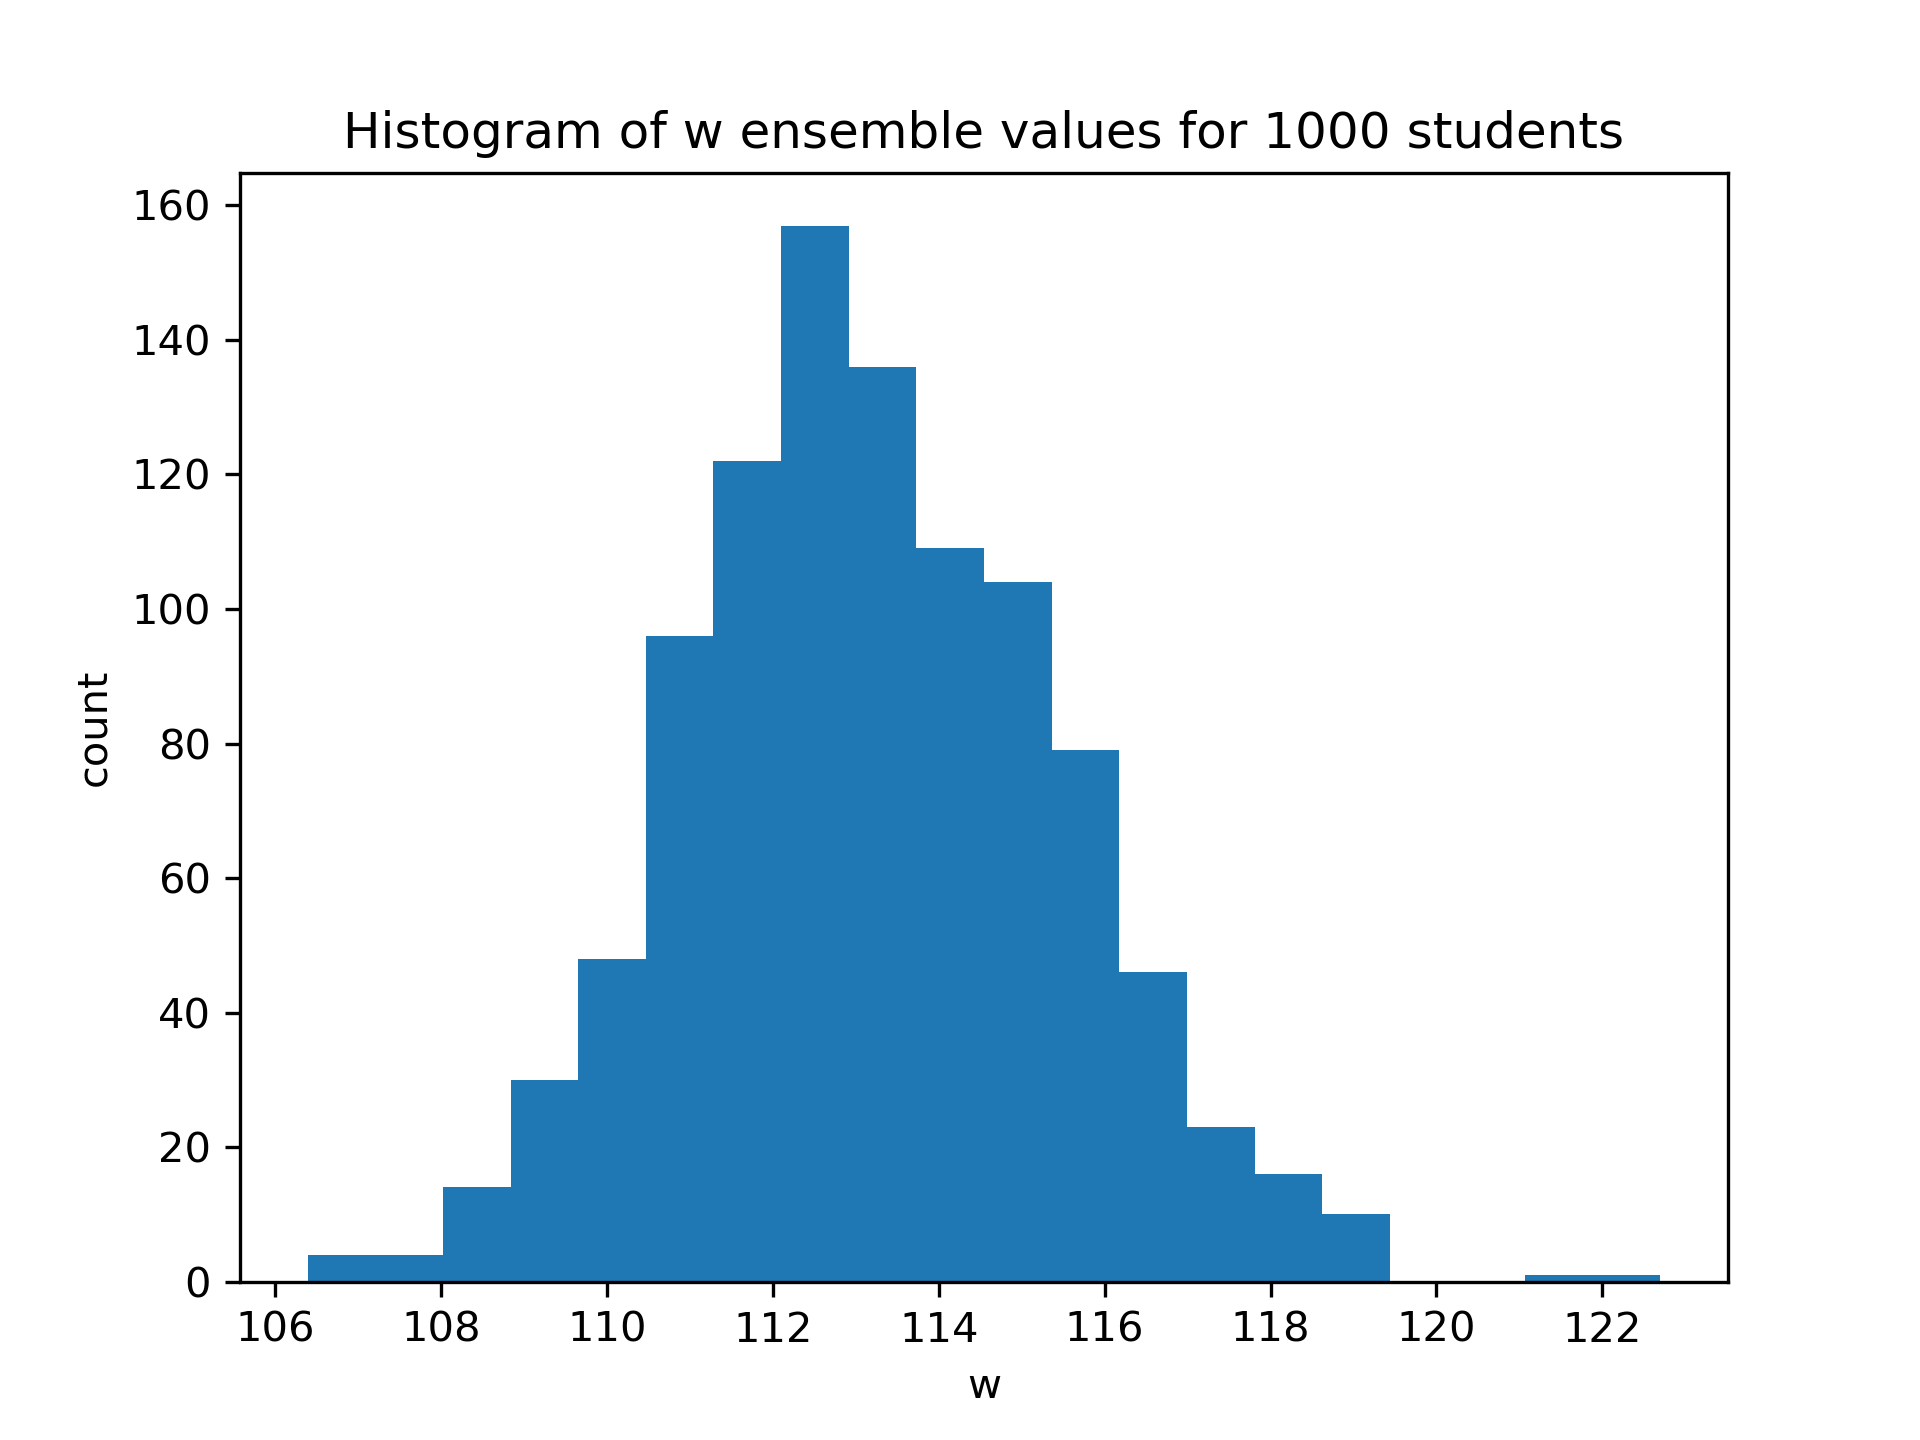
\includegraphics[scale=0.8]{./2_7.png}
        \end{center}
        The plot shows the distribution of the values of $w$ from each student.
        I picked 20 bins as there are roughly 20 integer value of $w$ that capture the majority of the normal distribution.

        There is some uncertainty in the $w$ (or the histogram's mean) which can be calculated as standard error like:
        \begin{equation}
            \sigma_{\bar{x}} = \frac{\sigma}{\sqrt{n}}
        \end{equation}
        Where $\sigma_{\bar{x}}$ is the standard error of the mean, $\sigma$ is the standard deviation of the sample and $n$ is the number of samples. \newline
        Using this equation we can calculate the standard error of the mean of the histogram as:
        \begin{equation}
            \sigma_{\bar{x}} = \frac{2.278191315242165}{\sqrt{1000}} = 0.07204273501779916
        \end{equation}
        
\end{document}
